\documentclass{minimal}
\usepackage{tikz}
\usetikzlibrary{
	calc, trees, positioning, arrows, chains, shapes.geometric,%
	decorations.pathreplacing, decorations.pathmorphing, shapes,%
	matrix, shapes.symbols
}

\tikzset{
	>=stealth',
 	punktchain/.style={
    rectangle, 
    rounded corners, 
    % fill=black!10,
    draw=black,
    very thick,
    text width=200pt, 
    minimum height=25pt,
    text centered, 
    on chain},
  line/.style={draw, thick, <-},
  element/.style={
    tape,
    top color=white,
    bottom color=blue!50!black!60!,
    minimum width=8em,
    draw=blue!40!black!90,
    very thick,
    text width=10em, 
    minimum height=3.5em, 
    text centered, 
    on chain},
  every join/.style={->, thick,shorten >=1pt},
  decoration={brace},
  tuborg/.style={decorate},
  tubnode/.style={midway, right=2pt},
}

\begin{document}
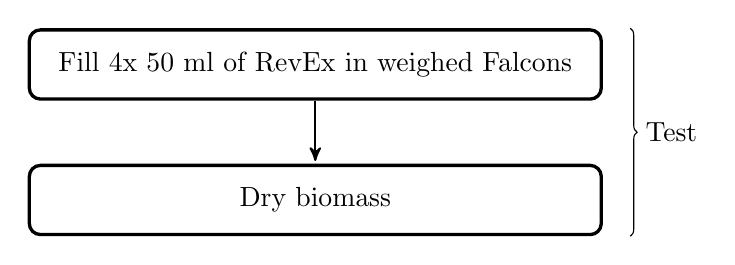
\begin{tikzpicture}[node distance=.8cm, start chain=going below,]
	\node [punktchain, join] (p1)	{Fill 4x 50 ml of RevEx in weighed Falcons};
	\node [punktchain, join] (p2)	{Dry biomass};

	\draw 	[tuborg, decoration={brace}] let \p1=(p1.north), \p2=(p2.south) in
			($(4, \y1)$) -- ($(4, \y2)$) node[tubnode] {Test};
\end{tikzpicture}
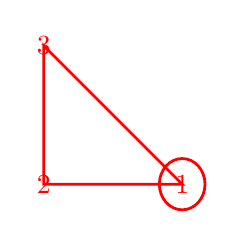
\begin{tikzpicture}
	\draw [line width=1pt, color=red] (50pt, 0pt) node[ellipse, draw] {1} -> (0pt, 0pt) node {2} -> (0pt, 50pt) node {3} -> cycle;
\end{tikzpicture}
\end{document}